% Options for packages loaded elsewhere
\PassOptionsToPackage{unicode}{hyperref}
\PassOptionsToPackage{hyphens}{url}
\PassOptionsToPackage{dvipsnames,svgnames*,x11names*}{xcolor}
%
\documentclass[
  10pt,
]{article}
\usepackage{amsmath,amssymb}
\usepackage{lmodern}
\usepackage{ifxetex,ifluatex}
\ifnum 0\ifxetex 1\fi\ifluatex 1\fi=0 % if pdftex
  \usepackage[T1]{fontenc}
  \usepackage[utf8]{inputenc}
  \usepackage{textcomp} % provide euro and other symbols
\else % if luatex or xetex
  \usepackage{unicode-math}
  \defaultfontfeatures{Scale=MatchLowercase}
  \defaultfontfeatures[\rmfamily]{Ligatures=TeX,Scale=1}
\fi
% Use upquote if available, for straight quotes in verbatim environments
\IfFileExists{upquote.sty}{\usepackage{upquote}}{}
\IfFileExists{microtype.sty}{% use microtype if available
  \usepackage[]{microtype}
  \UseMicrotypeSet[protrusion]{basicmath} % disable protrusion for tt fonts
}{}
\makeatletter
\@ifundefined{KOMAClassName}{% if non-KOMA class
  \IfFileExists{parskip.sty}{%
    \usepackage{parskip}
  }{% else
    \setlength{\parindent}{0pt}
    \setlength{\parskip}{6pt plus 2pt minus 1pt}}
}{% if KOMA class
  \KOMAoptions{parskip=half}}
\makeatother
\usepackage{xcolor}
\IfFileExists{xurl.sty}{\usepackage{xurl}}{} % add URL line breaks if available
\IfFileExists{bookmark.sty}{\usepackage{bookmark}}{\usepackage{hyperref}}
\hypersetup{
  colorlinks=true,
  linkcolor=Maroon,
  filecolor=Maroon,
  citecolor=Blue,
  urlcolor=blue,
  pdfcreator={LaTeX via pandoc}}
\urlstyle{same} % disable monospaced font for URLs
\usepackage[left=2cm, right=2cm, top=2cm, bottom=3cm, footskip =
.5cm]{geometry}
\usepackage{graphicx}
\makeatletter
\def\maxwidth{\ifdim\Gin@nat@width>\linewidth\linewidth\else\Gin@nat@width\fi}
\def\maxheight{\ifdim\Gin@nat@height>\textheight\textheight\else\Gin@nat@height\fi}
\makeatother
% Scale images if necessary, so that they will not overflow the page
% margins by default, and it is still possible to overwrite the defaults
% using explicit options in \includegraphics[width, height, ...]{}
\setkeys{Gin}{width=\maxwidth,height=\maxheight,keepaspectratio}
% Set default figure placement to htbp
\makeatletter
\def\fps@figure{htbp}
\makeatother
\setlength{\emergencystretch}{3em} % prevent overfull lines
\providecommand{\tightlist}{%
  \setlength{\itemsep}{0pt}\setlength{\parskip}{0pt}}
\setcounter{secnumdepth}{-\maxdimen} % remove section numbering
% Set up the fonts
\usepackage[urw-palatino]{mathdesign}
\usepackage[T1]{fontenc}


% Set the language for 508
\hypersetup{
  pdftitle = {title},
  pdflang = en-US}

% Add accessibility support from http://www.richschwinn.com/accessibility
\RequirePackage{accsupp}
\RequirePackage{pdfcomment}
\newcommand{\AccTool}[2]{\BeginAccSupp{method=pdfstringdef,unicode,Alt={{#1}}}\pdftooltip{{#2}}{{#1}}\EndAccSupp{}}


% Set up the headers and footers
\usepackage{graphicx}
\usepackage{fancyhdr}
\usepackage{ifthen}
%\usepackage{everypage-1x}
\usepackage{float}
%\usepackage{subfig}
%\usepackage{subcaption}

% Avoid struggling over figure and table float in Rmarkdown
\let\origfigure\figure
\let\endorigfigure\endfigure
\renewenvironment{figure}[1][2] {
    \expandafter\origfigure\expandafter[H]
} {
    \endorigfigure
}

\let\origtable\table
\let\endorigtable\endtable
\renewenvironment{table}[1][2] {
    \expandafter\origtable\expandafter[H]
} {
    \endorigtable
}

% First page has the large title and NOAA logo
\pagestyle{fancy}
\fancyhf{}
\setlength\headheight{40pt}
\fancyheadoffset[L]{0.5cm}
\cfoot{\thepage}

\fancyheadinit{%
   \ifthenelse{\value{page}=1}%
      {\fancyhead[R]{\textsf{\emph{March 9, 2022}}}
       \fancyhead[L]{\textsf{\LARGE SSC Ecosystem Working Group Report: March 2022}}
      }%
      {\fancyhead[R]{}
       \fancyhead[L]{\textsf{\emph{SSC Ecosystem Working Group Report: March 2022}}}
      }
}

\renewcommand{\headrulewidth}{0.4pt}
\renewcommand{\footrulewidth}{0pt}

% Make caption fonts a bit smaller
\usepackage[font={small}]{caption}


% Change section labels to san serif
\usepackage{sectsty}
\allsectionsfont{\normalfont\sffamily\bfseries}
\usepackage{booktabs}
\usepackage{longtable}
\usepackage{array}
\usepackage{multirow}
\usepackage{wrapfig}
\usepackage{float}
\usepackage{colortbl}
\usepackage{pdflscape}
\usepackage{tabu}
\usepackage{threeparttable}
\usepackage{threeparttablex}
\usepackage[normalem]{ulem}
\usepackage{makecell}
\usepackage{xcolor}
\ifluatex
  \usepackage{selnolig}  % disable illegal ligatures
\fi

\author{}
\date{\vspace{-2.5em}}

\begin{document}

The MAFMC SSC Ecosystem Working Group (WG) was established in May 2021
to assist the Council in developing short term and long term objectives
to advance the operational use of ecosystem information in management
decisions. As reported in
\href{https://www.mafmc.org/s/b_Ecosystem-WG_Proposed-Tasks-August-2021.pdf}{September
2021}, the WG has identified three general objectives:

\begin{enumerate}
\def\labelenumi{\arabic{enumi}.}
\tightlist
\item
  Expanding and clarifying the ecosystem portion of the SSC OFL CV
  determination process (short term objective)
\item
  Developing prototype processes to provide multispecies and system
  level scientific advice appropriate for Council decision making, in
  particular where there are multispecies and multifleet tradeoffs
  linking directly to economic and social outcomes (long term objective)
\item
  Collaborating with SSC species leads, stock assessment leads, and
  relevant working groups in developing the stock-specific Ecosystem and
  Socio-economic Profiles (ESP) process to specify stock-specific
  Ecosystem ToRs that are impactful and can be integrated into
  assessments (moderate-term objective)
\end{enumerate}

Objectives 1 and 3 aim to integrate appropriate ecosystem information at
the stock level of management decision making, while objective 2 applies
to current Council EAFM processes and potential future multispecies and
system level objectives.

Intended outcomes of WG work for the Council include: * An OFL CV
process that makes better use of ecosystem information in determining
the ABC * Evaluation of multiple ecosystem indicators and potential
development of thresholds for use in a revised EAFM risk assessment
and/or other Council processes * Increased range of opportunities for
relevant ecosystem information to be considered in management decision
processes

The WG has met four times since September 2021 (October, November,
December 2021 and January 2022) to outline the following work plans for
each objective.

\hypertarget{ecosystem-criteria-for-ofl-cv-determination}{%
\subsection{Ecosystem criteria for OFL CV
determination}\label{ecosystem-criteria-for-ofl-cv-determination}}

The WG focused on this objective in all four meetings. An initial step
was outlining an SSC decision process for evaluating stock level
ecosystem effects (Fig. \ref{fig:OFLCV}).

\begin{figure}

{\centering 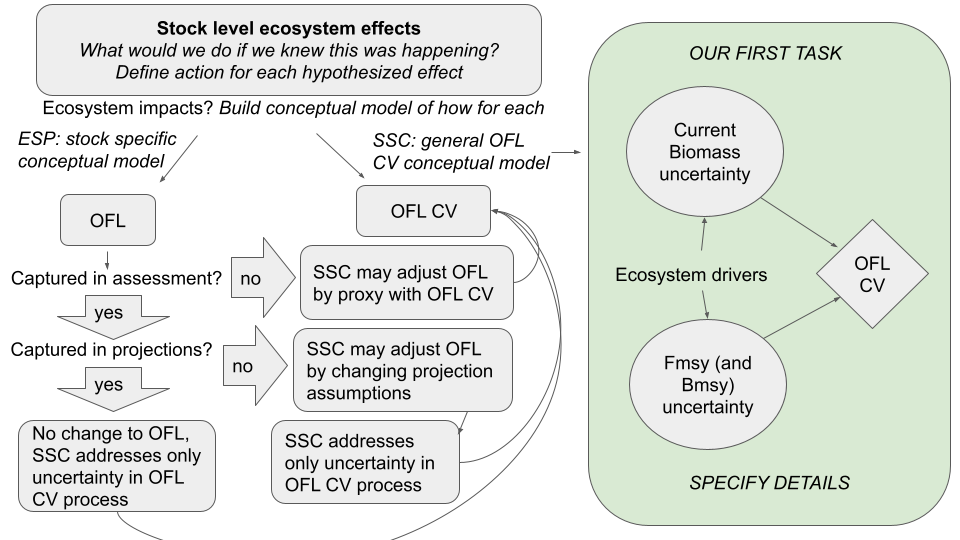
\includegraphics[width=1\linewidth]{images/OFLCVprocess} 

}

\caption{SSC process for incorporating ecosystem information into OFL CV decisions.}\label{fig:OFLCV}
\end{figure}

The WG outlined decisions for OFL CV centered on management responses.
How would we manage differently if we knew the following attributes of a
stock were changing?\\
* M is increasing/decreasing * Recruitment is in a low/high regime *
Growth rates are increasing/decreasing * Fish are maturing earlier/later
age or smaller/larger size * Sex ratio is changing * Spatial
distribution is changing

Other considerations are: Over what timeframe is change observed? Can we
expect change to continue? Overall, to the extent possible the goal is
to link changes to specific ecosystem factors to tease out expectations.

The WG outlined next steps and is currently designing analyses to
address a subset of these questions.

\begin{itemize}
\tightlist
\item
  Flesh out OFL CV conceptual model (Fig. \ref{fig:OFLCV}) as it relates
  to these and other parameters
\item
  Use Wiedenmann MSE framework to evaluate impact of changes in these
  parameters on OFL (assessment and projection) and or OFL CV, and
  performance of current HCR over multiple stocks already included in
  that model
\item
  Continue coordination with stock-specific conceptual model development
  and current assessments through research track working groups/ESP
  process
\end{itemize}

At the January 2022 meeting, WG member Mike Wilberg reported that he
(and students, UMD) will collaborate with John Wiedenmann (and students,
Rutgers) to implement the MSE framework for 2 species to start, focusing
on recruitment as the response. Summer flounder and Atlantic Mackerel
are proposed, with the groups to start with summer flounder. The plan
was to start towards the end of February 2022 with the students by
introducing the project, what the overall goals are, and get them up to
speed on code. Initial tasks include updating the MSE model with recent
stock assessment information. The WG discussed what scenarios to run,
and what kind of climate forcing to use. The students will be invited to
present to the WG and join discussions as the project progresses.

\hypertarget{ecosystem-indicator-evaluation-and-threshold-analyses}{%
\subsection{Ecosystem indicator evaluation and threshold
analyses}\label{ecosystem-indicator-evaluation-and-threshold-analyses}}

The WG outlined general themes for this objective at all meetings, but
began discussing them in earnest at the January 2022 meeting. Initial
thoughts for ecosystem and multispecies level indicator evaluation were
outlined in October-November 2021 (Fig. \ref{}fig:multispp).

\begin{figure}

{\centering 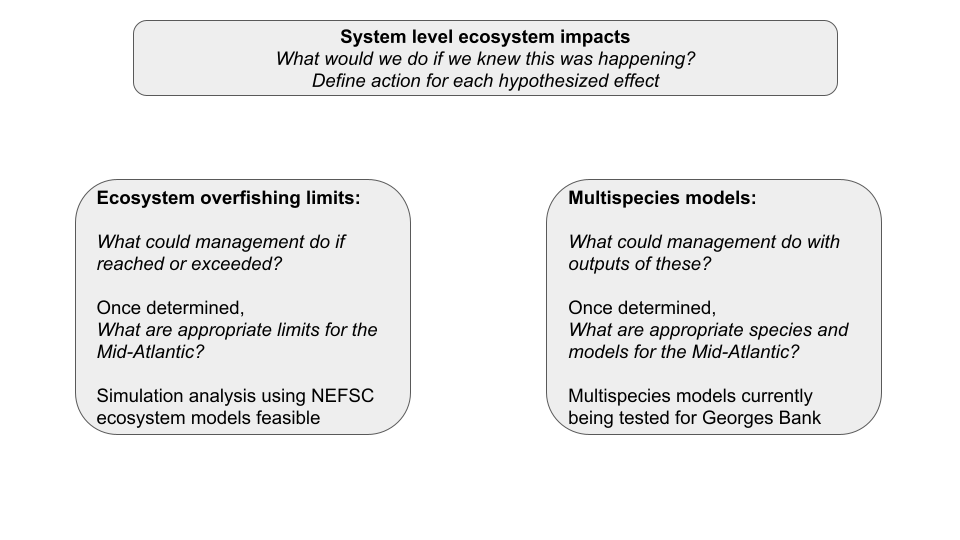
\includegraphics[width=1\linewidth]{images/multisppecosystem} 

}

\caption{SSC outline incorporating ecosystem information into multispecies and ecosystem decisions.}\label{fig:multispp}
\end{figure}

These tasks would require engagement with and guidance from the Council.
Funding has recently been secured within NEFSC to support these
analyses; Andy Beet (NEFSC), an experienced statistician and modeler who
currently contributes to the SOE, will work with the SSC and attend WG
meetings. While tasks have yet to be outlined, there are several
analyses that would address previous SSC and Council requests related to
EAFM and the SOE.

\begin{itemize}
\tightlist
\item
  For EAFM risk assessment, tasks could include

  \begin{itemize}
  \tightlist
  \item
    Develop additional risk elements
  \item
    Review and improve current indicators, risk criteria and identify
    potential thresholds
  \item
    WG noted this could also feed back into OFL CV ecosystem criteria
  \end{itemize}
\item
  Developing future decision making processes making best use of
  ecosystem (including social and economic) information could include

  \begin{itemize}
  \tightlist
  \item
    Ecosystem level reference points
  \item
    Multispecies decisions/reference points
  \end{itemize}
\end{itemize}

At the January 2022 meeting, the WG reviewed example multispecies
indicators, including the stock productivity indicator in the SOE (Fig.
\ref{fig:productivity-anomaly}) and similar indicators based on recent
stock assessments
(\url{https://sgaichas.github.io/stockstatusindicator/MultisppRec.html}).

\begin{figure}

{\centering \includegraphics{March2022_SSCEcoWG_files/figure-latex/productivity-anomaly-1} 

}

\caption{Small fish per large fish biomass anomaly in the Mid-Atlantic Bight. The summed anomaly across species is shown by the black line.}\label{fig:productivity-anomaly}
\end{figure}

The ecosystem overfishing (EOF) indicators presented in the 2021 SOE
have been subject to several requests from both Councils for additional
analysis, including impacts of changes in phytoplankton community
composition, evaluation and comparison of theoretical and empirical
thresholds, and evaluation of ecosystem optimum yield (see 2022
\href{https://www.mafmc.org/s/b_SOE-Cover-letter-and-request-memo.pdf}{SOE
Request Memo}). The WG requested a detailed presentation of the current
EOF indicators at an upcoming meeting.

\hypertarget{collaboration-with-assessment-working-groupsesp-process}{%
\subsection{Collaboration with assessment working groups/ESP
process}\label{collaboration-with-assessment-working-groupsesp-process}}

WG members are involved with the \emph{Illex} (Paul Rago), black sea
bass (Gavin Fay), and bluefish (Sarah Gaichas) research track assessment
working groups and ecosystem ToRs/ESP processes.

The ESP is intended to provide ``a structured framework to incorporate
ecosystem and socioeconomic information into stock advice'' (Abby
Tyrell, NEFSC, presentation to the Bluefish research track WG, November
2021). The framework identifies important bottlenecks in the stock's
life history using literature review and conceptual modeling, identifies
and tests indicators linking ecosystem and socioeconomic conditions and
stock performance, and assesses whether conditions are favorable for the
stock based on the indicators. The ESP is intended to be included with
the stock assessment document as an appendix to the report.

The framework can be linked with assessment ToRs, as demonstrated by
Abby in Fig. \ref{fig:ESPex}).

\begin{figure}

{\centering 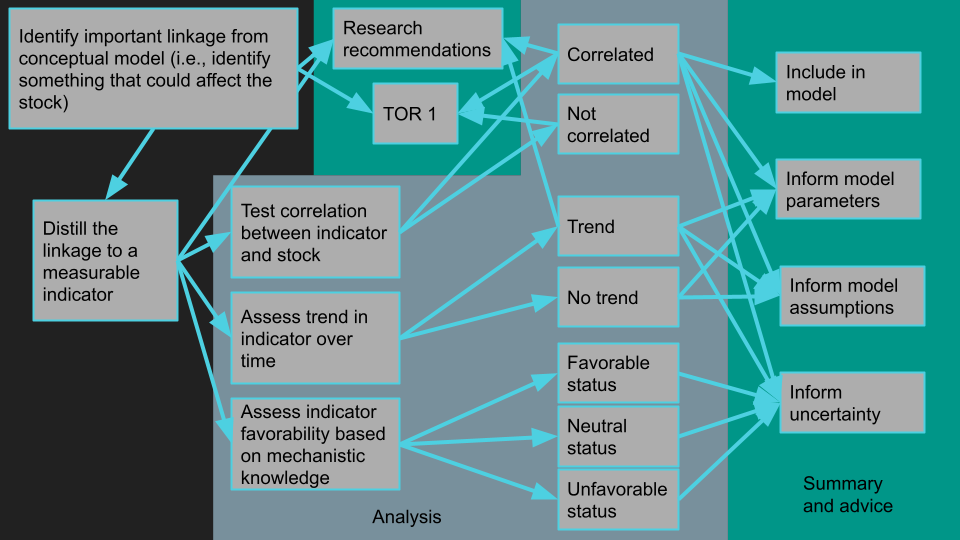
\includegraphics[width=1\linewidth]{images/bluefish esp update 11-18-21} 

}

\caption{Example flow of information in the bluefish ESP, Abby Tyrell, November 2021}\label{fig:ESPex}
\end{figure}

The WG notes that ESP information can be used by the SSC in many ways.
Even if not specifically included in the assessment model, ESP
indicators could provide critical information regarding stock
implications and processes within an ecosystem context.

More detailed information on the ESP process can be provided to the SSC
at a future meeting.

The WG welcomes full SSC discussion of the points raised in this report,
and invites any other members to participate at any time. The next
meeting is tentatively scheduled for April 2022.

\end{document}
